\documentclass{article}
\usepackage{graphicx}
\usepackage{amsmath}
\usepackage{hyperref}

\title{Filters}
\author{Abhishek Amit Raje}
\date{November 2023}

\hypersetup{
    colorlinks=true,
    linkcolor=red,
    urlcolor=red
}

\begin{document}

\begin{titlepage}
  \centering
  
\includegraphics[width=0.4\textwidth]{iithlogo.png}\par\vspace{1cm}
  {\scshape\LARGE Indian Institute of Technology Hyderabad \par}
  \vspace{1cm}
  {\scshape\Large Analog Electronics and Integrated Circuits \par}
  \vspace{1.5cm}
  \maketitle
\end{titlepage}

\section{BandPass Filter with Sallen Key Topology}

\begin{figure}[ht]
  \centering
  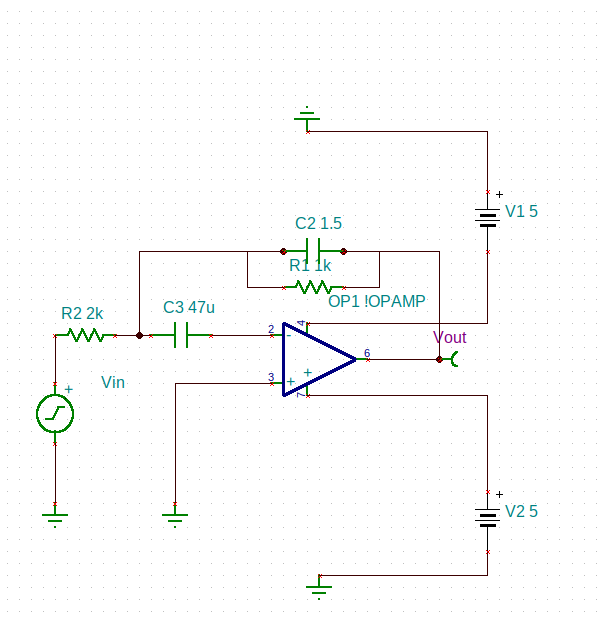
\includegraphics[width=0.6\linewidth]{bandpasscirc.png}
  \caption{Bandpass filter with Sallen Key Topology}
  \label{fig:circuit_simulation}
\end{figure}

\begin{figure}[ht]
  \centering
  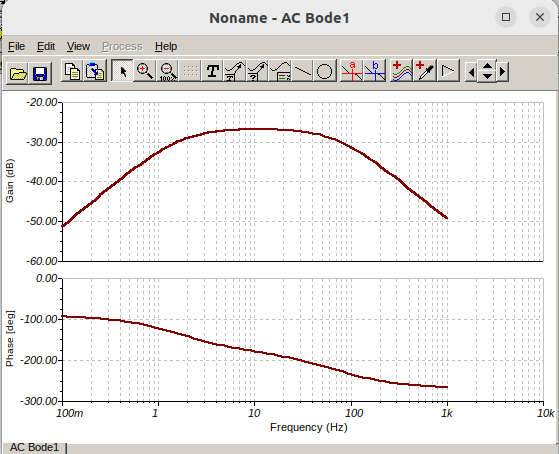
\includegraphics[width=0.5\linewidth]{BandPassbode.png}
  \caption{Bode Plot or AC Transfer Characteristics of the filter}
  \label{fig:bode_plot}
\end{figure}

\newpage

\begin{figure}[ht]
  \centering
  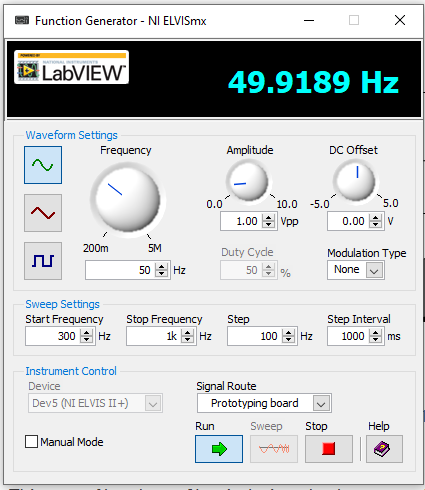
\includegraphics[width=0.5\linewidth]{BandPass50Hzfgen.png}
  \caption{Function generator input at 50Hz}
  \label{fig:input_50Hz}
\end{figure}

\begin{figure}[ht]
  \centering
  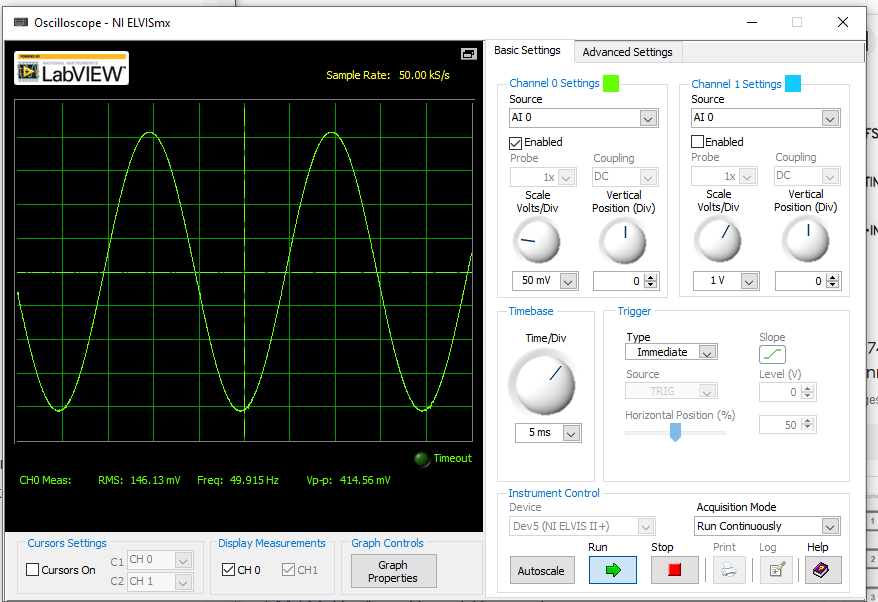
\includegraphics[width=0.6\linewidth]{BandPass50HzScope.png}
  \caption{Output signal at 50Hz}
  \label{fig:output_50Hz}
\end{figure}

\newpage

\begin{figure}[ht]
  \centering
  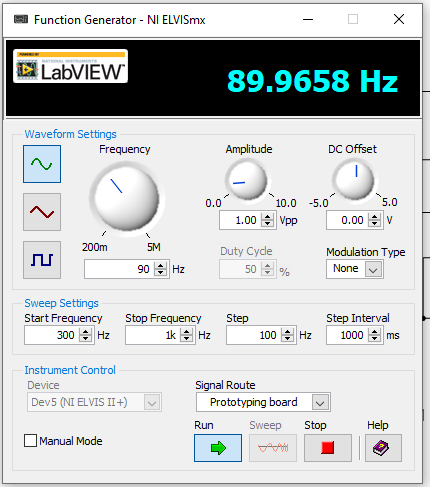
\includegraphics[width=0.5\linewidth]{BandPass90Hzfgen.png}
  \caption{Function generator input at 90Hz}
  \label{fig:input_90Hz}
\end{figure}

\begin{figure}[ht]
  \centering
  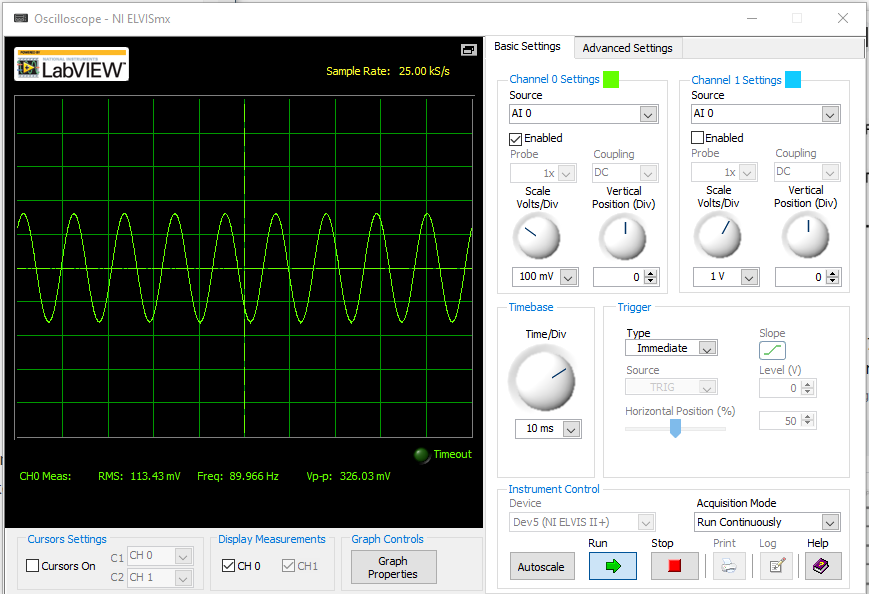
\includegraphics[width=0.6\linewidth]{BandPass90HzScope.png}
  \caption{Output signal at 90Hz}
  \label{fig:output_90Hz}
\end{figure}

\newpage

\begin{figure}[ht]
  \centering
  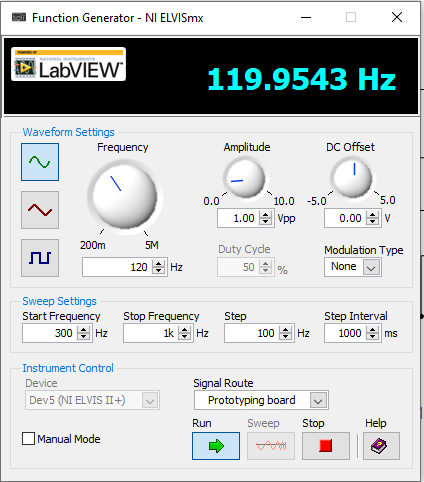
\includegraphics[width=0.5\linewidth]{BandPass120Hzfgen.png}
  \caption{Function generator input at 120Hz}
  \label{fig:input_120Hz}
\end{figure}

\begin{figure}[ht]
  \centering
  \includegraphics[width=0.65\linewidth]{BandPass120HzScope.png}
  \caption{Output signal at 120Hz}
  \label{fig:output_120Hz}
\end{figure}

\newpage

Since the circuit used is of the second order, the roll-off rate is 40 dB/decade. The decrease in amplitude can be explained by the magnitude of the bode plot, which is always less, thus showing attenuation of the input signal.

The phase shift can also be explained by the phase part of the bode plot:
\[
f_0 = \frac{1}{2\pi \sqrt{R_1 R_2 C_1 C_2}}
\]

For the given values:
\[
f_0 = 10 \, \text{Hz}
\quad
f_l = 1 \, \text{Hz}
\quad
f_h = 100 \, \text{Hz}
\]

\[
Q = \frac{1}{3 - \frac{R_2}{R_1}}
\]

For the given values:
\[
Q = 0.5
\]

The higher the quality factor, the more the roll-off rate. This can be observed from the rate of decrease of the slope of the magnitude of the bode plot after the cutoff frequency of 1Hz and 100Hz.

The transfer function and the stability of the poles will be explained later in the doc
\newpage
\section{Low Pass Filter with Sallen Key Topology}
\begin{figure}[ht]
  \centering
  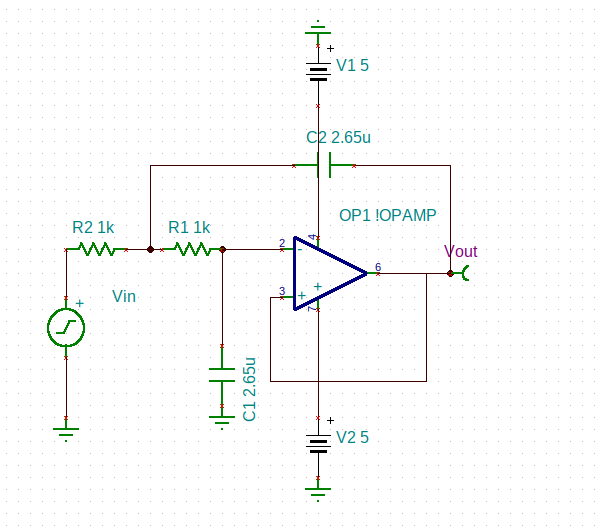
\includegraphics[width=0.6\linewidth]{lowpasscirc.png}
  \caption{Low Pass Circuit}
  \label{fig:output_120Hz}
\end{figure}

\begin{figure}[ht]
  \centering
  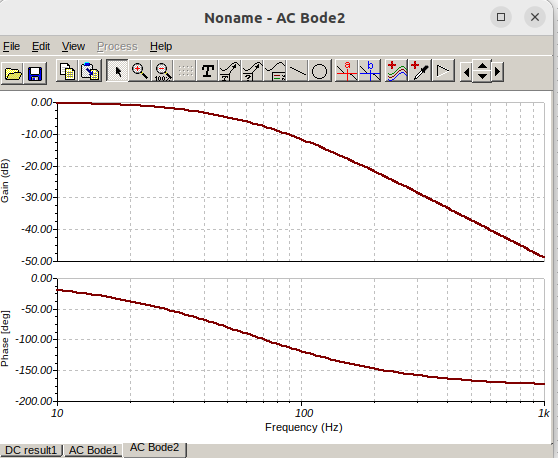
\includegraphics[width=0.6\linewidth]{lowpassbode.png}
  \caption{AC Transfer Characteristics of Low Pass Filter}
  \label{fig:output_120Hz}
\end{figure}
\newpage

\[
f_0 = \frac{1}{2\pi \sqrt{R_1 R_2 C_1 C_2}}
\]

The following inferences can be made from the bode plot:

The magnitude of the bode plot explains the attenuation of the output signal on increasing frequency, thus showing its low pass characteristics.

The phase shift character is seen to be more or less linear. Since it is an implementation of a second-order filter, the roll-off rate is 40dB/decade.
\begin{figure}[ht]
  \centering
  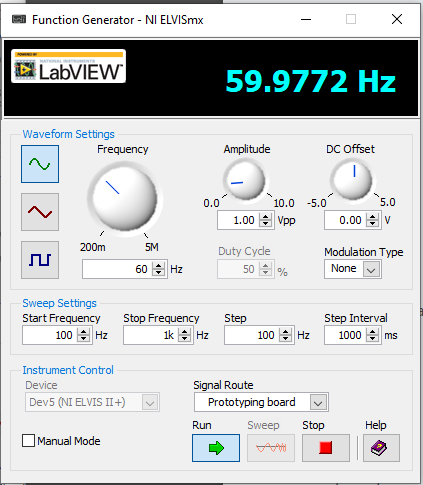
\includegraphics[width=0.5\linewidth]{lowpass60Hzfgen.png}
  \caption{Function generator input at 60Hz}
  \label{fig:output_120Hz}
\end{figure}
\begin{figure}[ht]
  \centering
  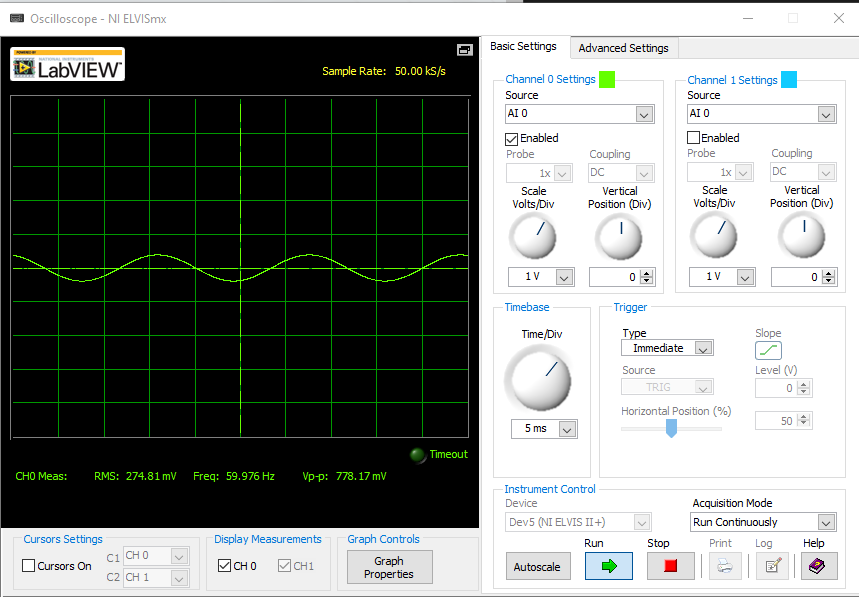
\includegraphics[width=0.6\linewidth]{lowpass60Hzscope.png}
  \caption{ Signal}
  \label{fig:output_120Hz}
\end{figure}
\begin{figure}[ht]
  \centering
  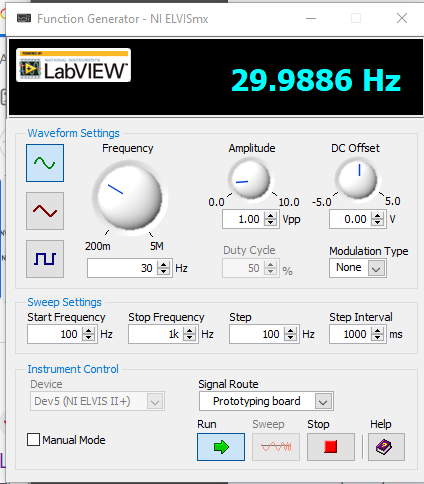
\includegraphics[width=0.6\linewidth]{lowpass30Hzfgen.png}
  \caption{Function generator input at 30Hz}
  \label{fig:output_120Hz}
\end{figure}
\begin{figure}[ht]
  \centering
  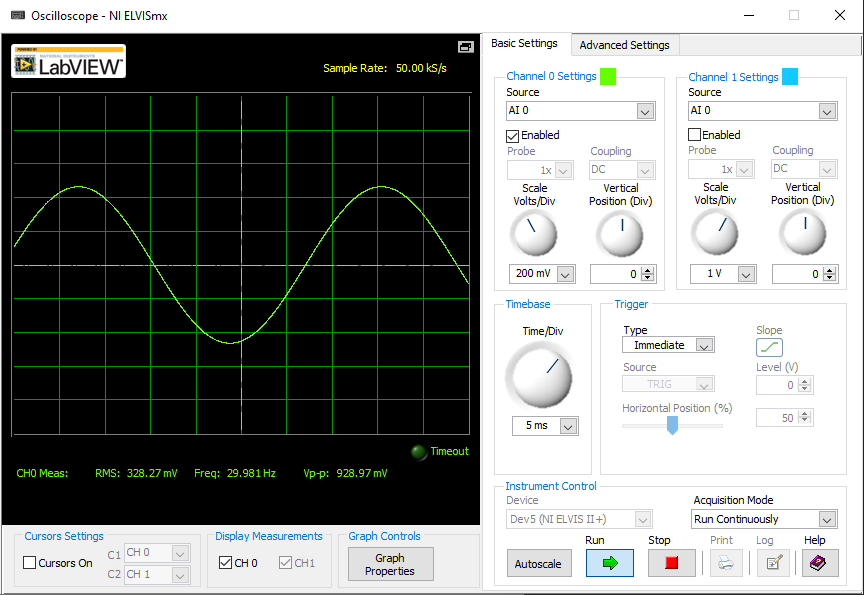
\includegraphics[width=0.7\linewidth]{lowpass30Hzscope.png}
  \caption{ Signal}
  \label{fig:output_120Hz}
\end{figure}
\begin{figure}[ht]
  \centering
  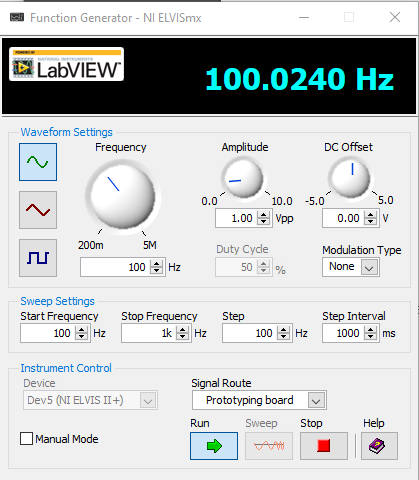
\includegraphics[width=0.6\linewidth]{lowpass100Hzfgen.png}
  \caption{Function generator input at 100Hz}
  \label{fig:output_120Hz}
\end{figure}
\begin{figure}[ht]
  \centering
  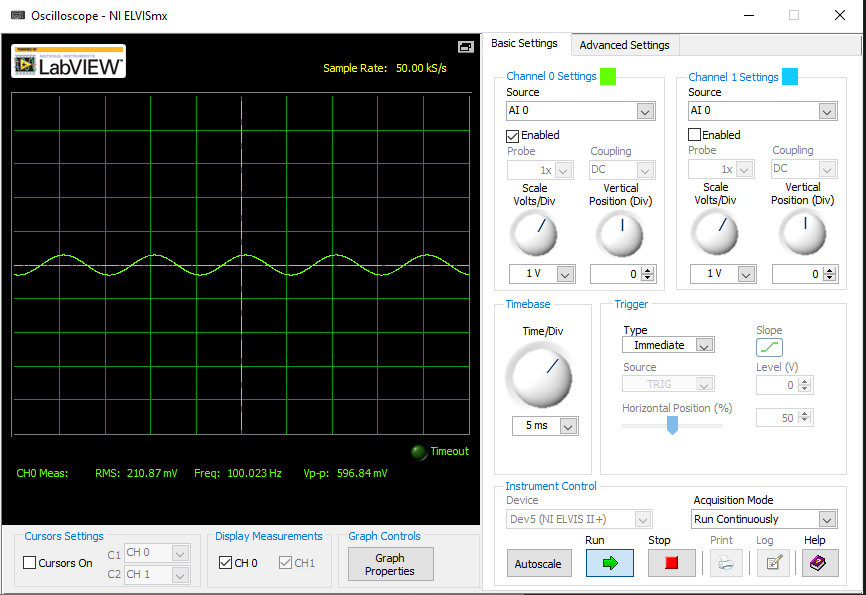
\includegraphics[width=0.7\linewidth]{lowpass100Hzscope.png}
  \caption{ Signal}
  \label{fig:output_120Hz}
\end{figure}
\end{document}
